\documentclass[a4paper, 12pt]{article}

%\usepackage{natbib}
\usepackage[english]{babel}
\usepackage{amsmath, amssymb}
\usepackage{parskip}
\usepackage{graphicx}

\begin{document}

\title{AA2 Practical Assignment}
\author{Maarten de Jonge, Koen Keune, Edwin Odijk,\\ Francesco Stablum, Marysia Winkels}
\maketitle

\section*{Introduction}
%something something sampling based fitted Q-iteration/value-iteration, something something continuous
This report describes the extension on an old AA1 assignment for the AA2 course. The existing predator/prey game's environment was changed from discrete to continuous, and the game was optimized using sampling based fitted Q-iteration/value-iteration.%\cite{ng_lecture}\cite{musze}

FVI (Fitted Value Iteration) is an algorithm that is suited for
continuous state spaces with continuos features extracted from
the state. 
The value function of a certain state is inferred by
extracting at first the features $\phi(s^{(i)})$ 
after having sampled some states 
$s^{(1)}\ldots s^{(i)} \ldots s^{(m)}$, 
and then by fitting via linear regression
the respective estimated state values $y^{(i)}$ 
in order to obtain the vector
of weights $\theta$.

The estimated state values $y^{(i)}$ are calculated as follows:
for each action $a$ and state $s^{(i)}$, 
$k$ state transitions are performed by using probabilities from 
an MDP model.
An estimated $Q$-value for the $\langle a,s^{(i)}\rangle$ pair is obtained
by averaging the sums of rewards of $s^{(i)}$ and
discounted value of the
state obtained from the transition from $s^{(i)}$.
In this step the $V$-function from the previous iteration has been used,
which, at the first iteration, has been set to 0.

These estimated $Q$-values are then used in a Bellman-like 
backup operator which selects the highest $Q$-value across all actions,
and for the specific current $s^{(i)}$.
This will become the current estimated $V$-value for $s^{(i)}$. 
This value is denoted
by the symbol $y^{(i)}$ in order to highlight the fact that it's 
a quantity that is subject to regression.

Once all $y^{(\cdot)}$ values have been obtained,
the previosly mentioned regression is performed.
This whole procedure is performed iteratively for a pre-determined
number of iterations.

\section*{Implementation} 
%HOW IT'S MADE

\section*{Comparison of Algorithms}
%new implementations vs old results
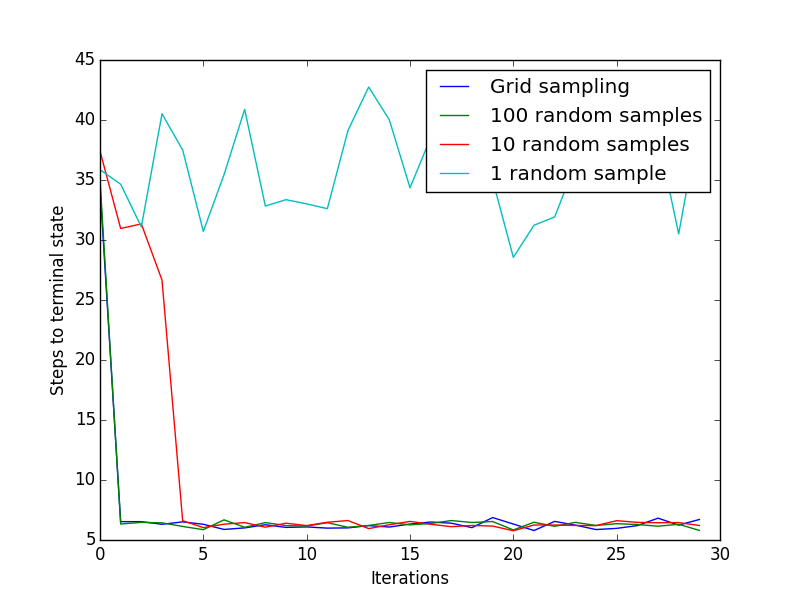
\includegraphics[scale=0.7]{convergence.png}
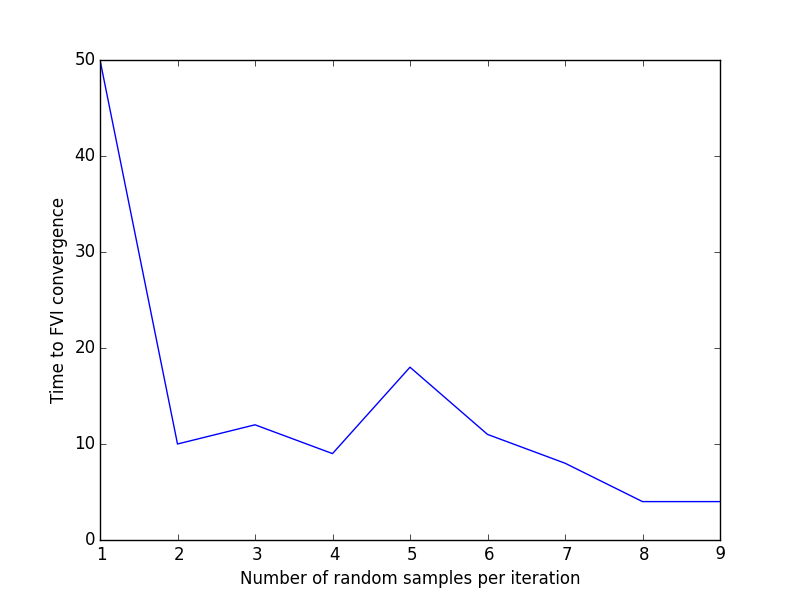
\includegraphics[scale=0.7]{n_samples.png}

\section*{Conclusion}
% ._.

\section*{References}
%\bibliographystyle{plain}
%\bibliography{ref}

\end{document}
